\documentclass[12pt,a4paper]{article}

\title{LABWORK 4 REPORT}
\author{Le Trung Nghia - USTHBI5-098 \\ \\ Ta Nguyen Long - USTHBI5-080 \\ \\ Do Huy Manh - USTHBI6-093 \\ \\ Nguyen Trong Nhan - USTHBI4-115}

\usepackage{listings}
\usepackage{color}
\usepackage{graphicx}
\usepackage[section]{placeins}
\usepackage{float}

\begin{document}
\maketitle
\newpage 
\section{Why Hadoop?}
- We choose Hadoop MapReduce framework because it breaks a large chunk into smaller ones and processed separately on different data nodes , then it collects the results from multiple nodes to return a single final result. Moreover, it has to read from and write to a disk which makes Hadoop MapReduce able to work with a very large data sets. Last but not least, Hadoop is an open source implementation of MapReduce programming model and it is available for Java.
\section{How?}
- First the input will be a text file that contains many sentences (with many words).
\begin{figure}[!htb]
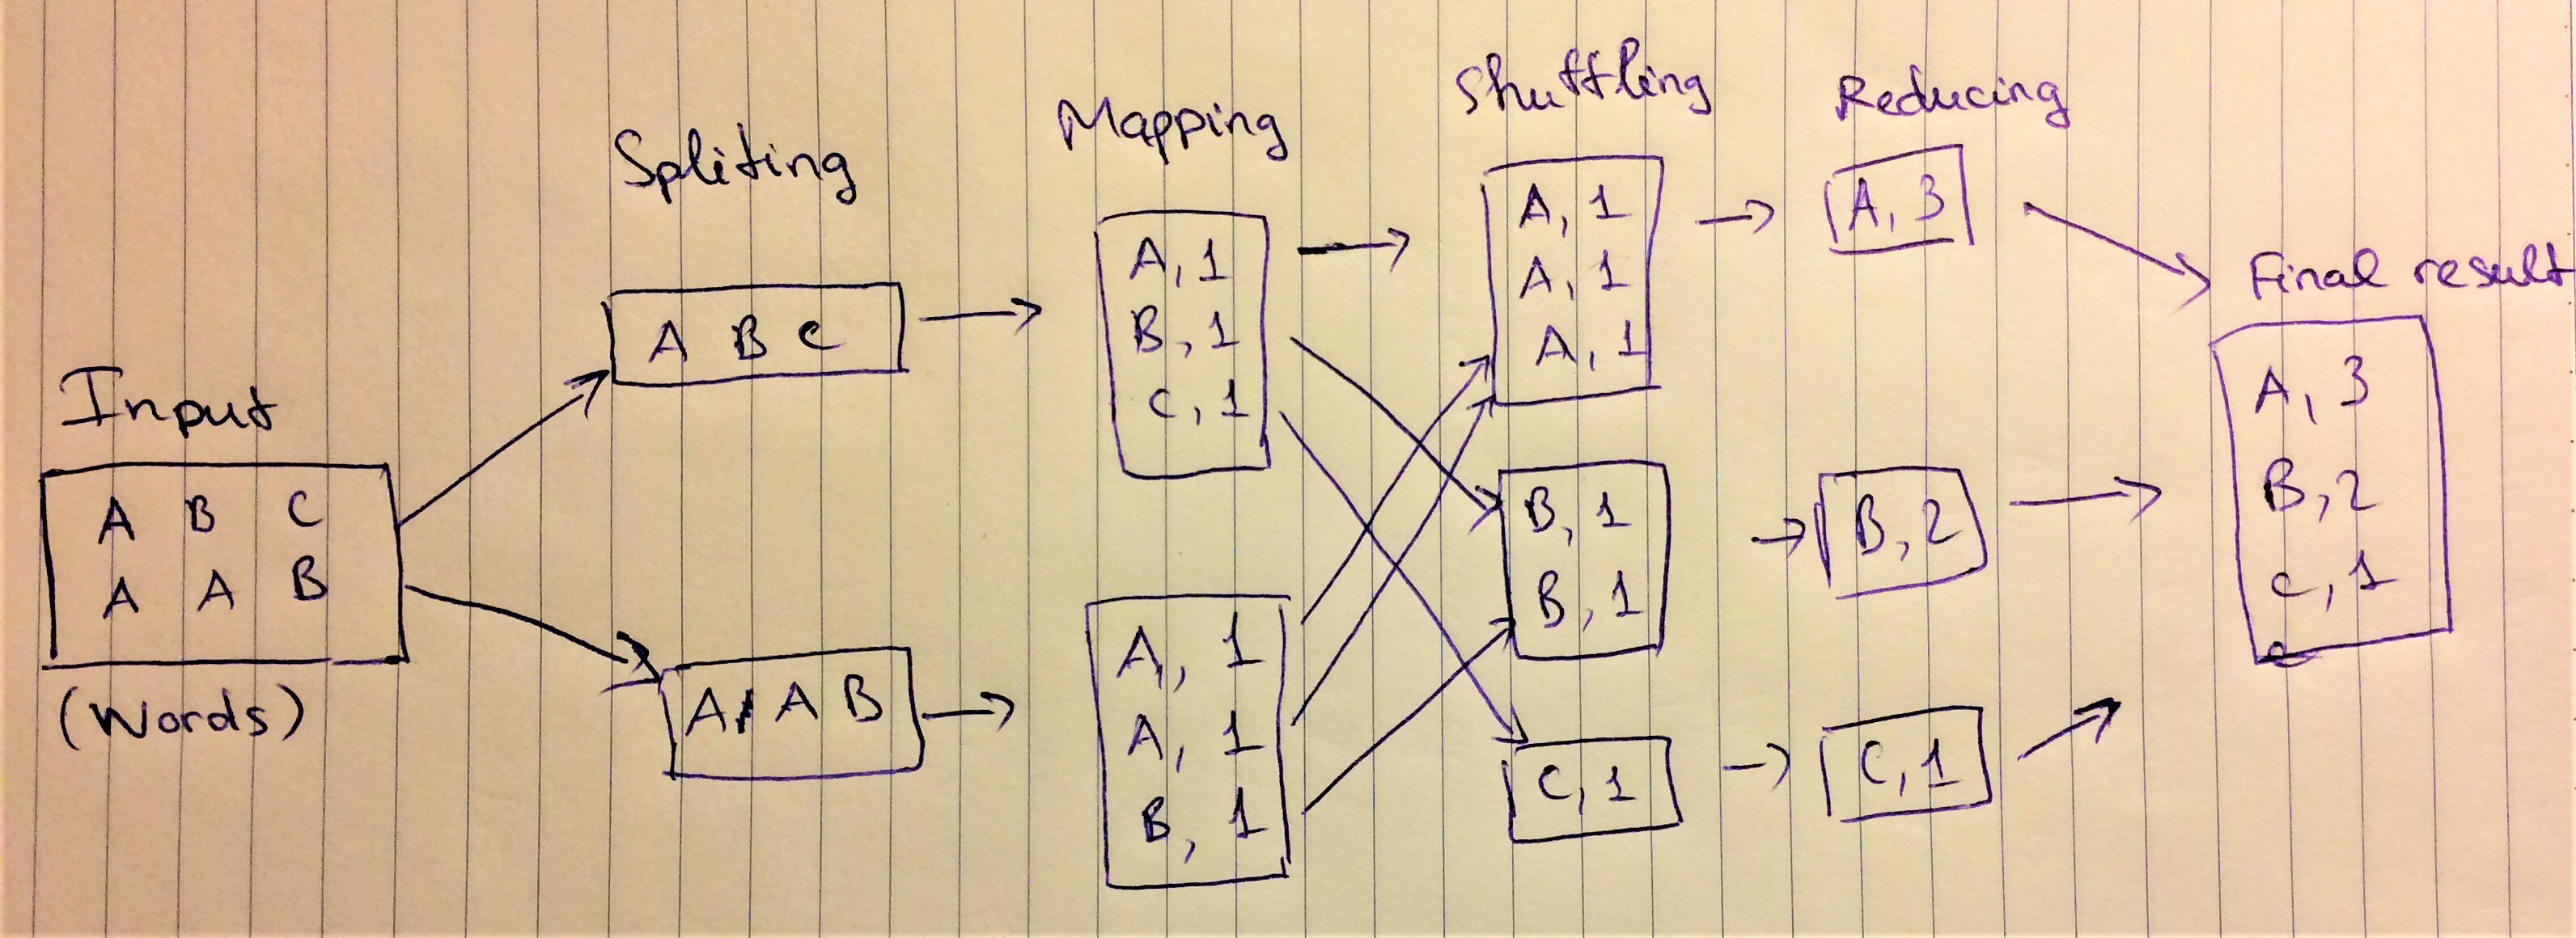
\includegraphics[width=\linewidth]{Mapper-Reducer.jpg}
\caption{Mapper - Reducer}
\end{figure}
\\ - The system will then break down the file and split it into different sentences (this is the step where different tasks will be assigned to different nodes). Then each node will do their job by breaking down the sentence and filtering each word in that sentence (this is the Mapping step). After the word has been filtered, it will be shuffled into different groups with each group contains the same word (this can be called the sort step). Finally, the Reducing step is where the counting process took place, it will count the number of words from each group to produce the final result. As can be seen from figure 1, the final result is the result of each group in the Reducing step.
\section{Who did what?}
- Code: Ta Nguyen Long. \\
- Report: Le Trung Nghia.
\end{document}
